\documentclass[12pt]{article}
\setlength{\parindent}{0pt}
\title{TEK5030 Project Report}
\usepackage[final]{pdfpages}
\usepackage{amsmath}
\usepackage{float}
\usepackage{graphicx}
\author{Bryan Walther, Didrik Samdanger, Carlos Ankour Navarro}
\usepackage[utf8]{inputenc} 
\usepackage{listings}
\usepackage{xcolor}
\usepackage{amssymb}
\graphicspath{ {./img/} }
\renewcommand\arraystretch{1.2}

\definecolor{codegreen}{rgb}{0,0.6,0}
\definecolor{codegray}{rgb}{0.5,0.5,0.5}
\definecolor{codepurple}{rgb}{0.58,0,0.82}
\definecolor{backcolour}{rgb}{0.95,0.95,0.92}

\usepackage{hyperref}
\hypersetup{
    colorlinks,
    citecolor=black,
    filecolor=black,
    linkcolor=black,
    urlcolor=black
}

\lstdefinestyle{mystyle}{
    backgroundcolor=\color{backcolour},   
    commentstyle=\color{codegreen},
    keywordstyle=\color{magenta},
    numberstyle=\tiny\color{codegray},
    stringstyle=\color{codepurple},
    basicstyle=\ttfamily\footnotesize,
    breakatwhitespace=false,         
    breaklines=true,                 
    captionpos=b,                    
    keepspaces=true,                 
    numbers=left,                    
    numbersep=5pt,                  
    showspaces=false,                
    showstringspaces=false,
    showtabs=false,                  
    tabsize=2
}

\lstset{style=mystyle}
\lstset{extendedchars=false}


\begin{document}
\maketitle

\section{Introduction}
Monocular depth estimation in computer vision is the problem of extracting depth information of a scene from single images captured by monocular cameras.
This is a challenging problem because the ability to perceive depth is achieved through stereo vision, which adds a constraint to the problem of estimating the depth.
In contrast, monocular depth estimation is an ill-posed problem, since we attempt to infer depth information of a scene using only visual cues of a single image.
Most modern approaches to monocular depth estimation involves using large datasets with labeled images to train deep learning models, where the ground truth depth information for each sample is included in the training set.
A popular model that does this is MiDaS, which is trained on up to 12 different datasets, and predicts the relative depth map for a given image.
However, the predicted depth maps only offer depth information up to scale, meaning that we face the issue of scale-ambiguity.
Some work has been done on attempting to learn the absolute depth of a scene, a notable example being ZoeDepth.
ZoeDepth attempts to learn depth information while also maintaining the metric scale.
After testing ZoeDepth however, we find that the accuracy of the model in predicting the true scale is generally poor.
\\ \\
In this project we attempt to tackle the problem of scale-ambiguity in estimated depth-maps by leveraging prior knowledge of the real world geometry of the scene.
As a proof of concept, we apply this idea to traffic footage, where the goal is to get good distance estimates from a dash-camera to any object in the scene.

\section{Methods}
\textbf{TODO: Explain the approach for getting the correct scale of a depth map by detecting license plates with known real world dimensions.}
\begin{figure}[H]
    \centering
    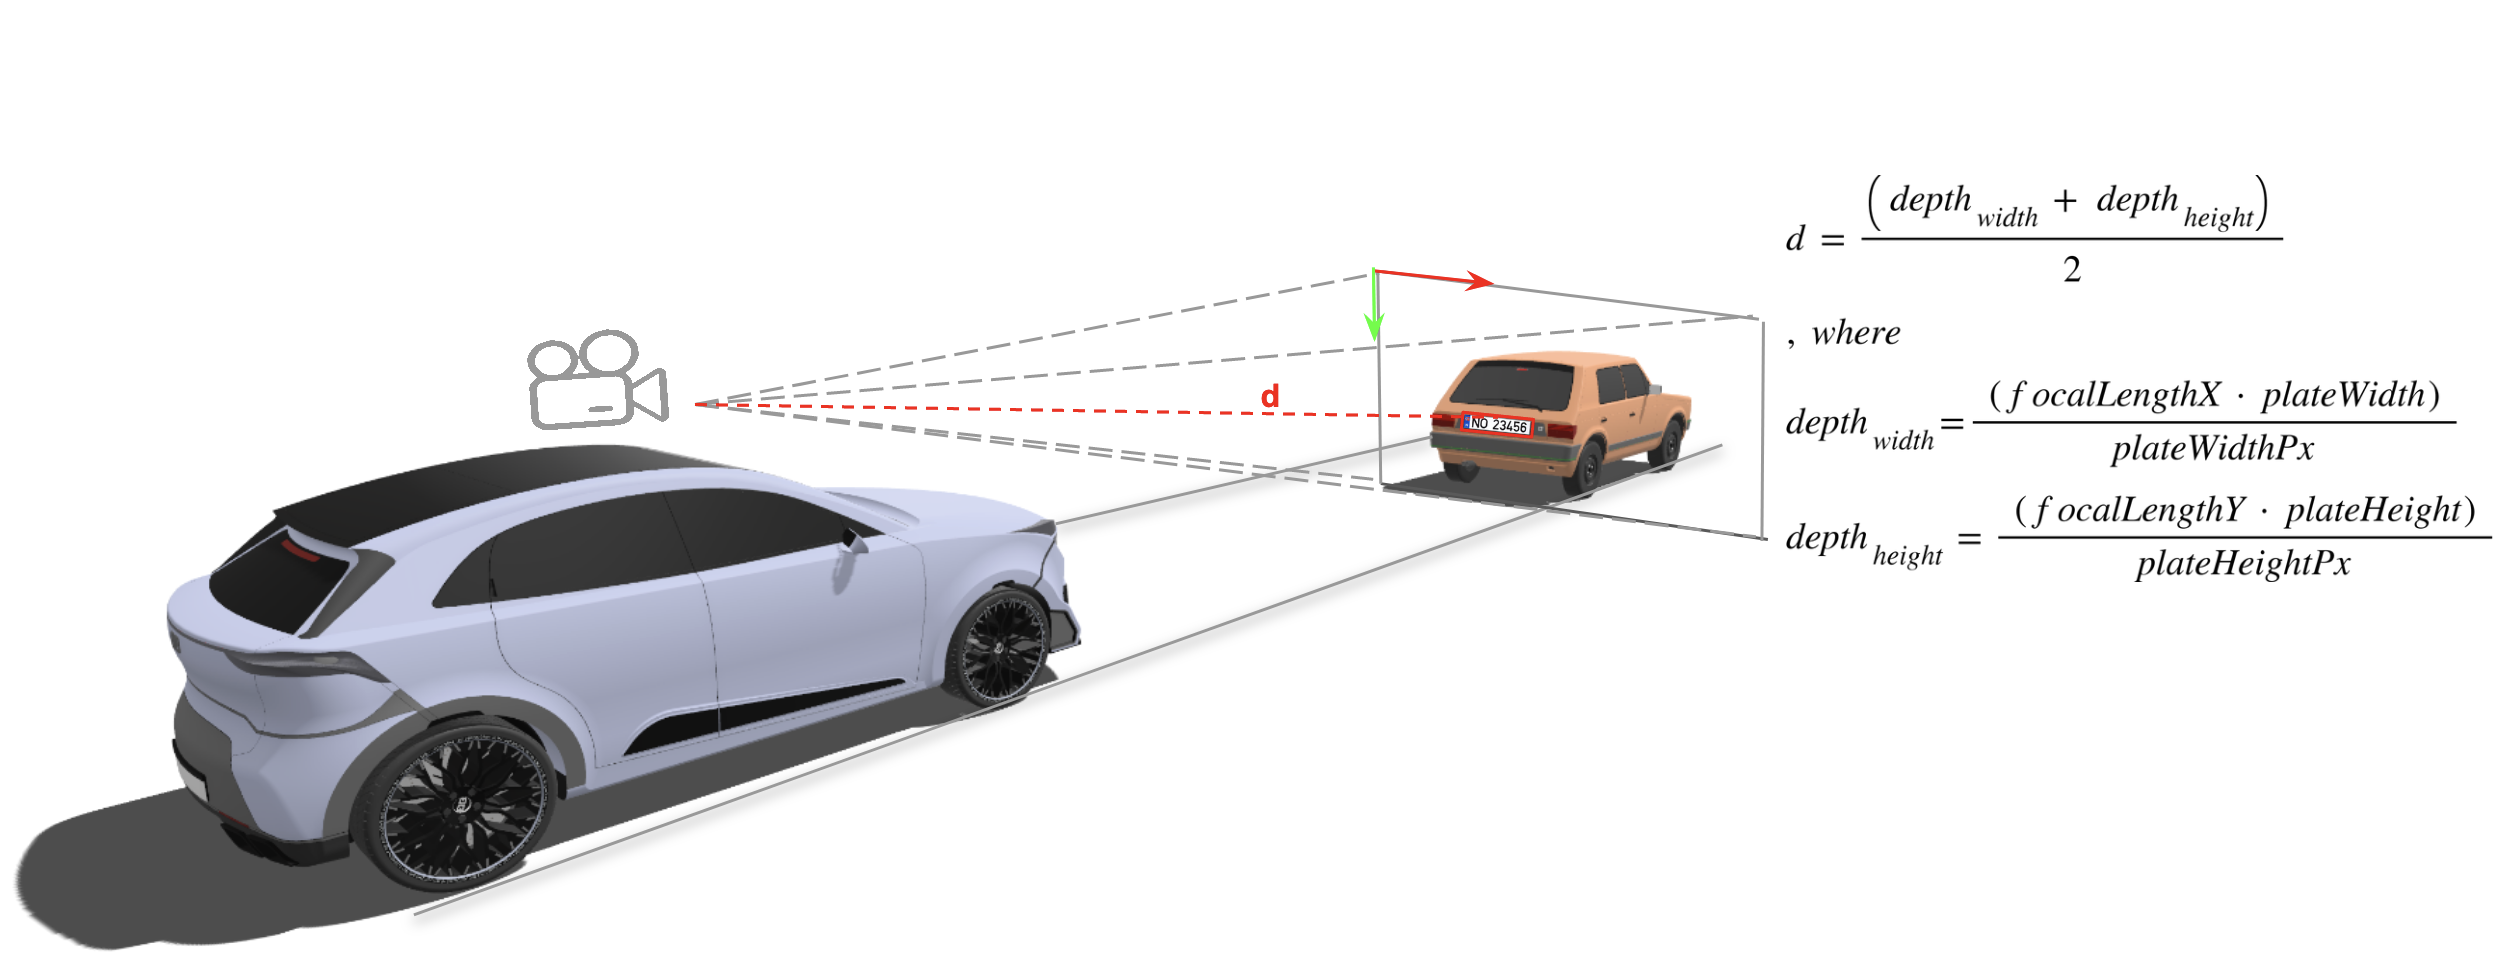
\includegraphics[width=1.0\textwidth]{img/illustration.png}
    \caption{Depth estimation of license plates }
    \label{fig:illustration}
\end{figure}

% Give outline of the procedure.
% Include images of the depth map from both MiDaS and ZoeDepth
% Mention how the ZoeDepth maps appear to have better resolution, which is why we chose these maps as initial maps.
% Mention the downside being that its much slower.
% Include images of the vehicle detections and the cropped images
\section{Results}
% Start by showing the parking lot example, where we already calibrate the camera and have the focal length.

% Show the dashcam example, explain we do not calibrate the camera, and only manually tweak the focal length until we get somewhat reasonable results.
% Only used to show a use case for this.
\section{Discussion}
% Explain how given we have a calibrated camera, and the focal length of the camera, the results seem pretty good for low precision use cases.
% Explain some of the issues:
%   - For this to work, we need good and stable license plate detections.
%   - The issue of perspective when viewing the license plates, could be resolved through filtering or perspective using homography.
%   - Cannot run realtime without a GPU
%   - Poorly optimized
\section{Conclusion}
% Just summarize the results and the discussion.
\end{document}

\end{document}
